% ----------------------------------------------------------------- %
%             The Speech Signal Processing Toolkit (SPTK)           %
%             developed by SPTK Working Group                       %
%             http://sp-tk.sourceforge.net/                         %
% ----------------------------------------------------------------- %
%                                                                   %
%  Copyright (c) 1984-2007  Tokyo Institute of Technology           %
%                           Interdisciplinary Graduate School of    %
%                           Science and Engineering                 %
%                                                                   %
%                1996-2017  Nagoya Institute of Technology          %
%                           Department of Computer Science          %
%                                                                   %
% All rights reserved.                                              %
%                                                                   %
% Redistribution and use in source and binary forms, with or        %
% without modification, are permitted provided that the following   %
% conditions are met:                                               %
%                                                                   %
% - Redistributions of source code must retain the above copyright  %
%   notice, this list of conditions and the following disclaimer.   %
% - Redistributions in binary form must reproduce the above         %
%   copyright notice, this list of conditions and the following     %
%   disclaimer in the documentation and/or other materials provided %
%   with the distribution.                                          %
% - Neither the name of the SPTK working group nor the names of its %
%   contributors may be used to endorse or promote products derived %
%   from this software without specific prior written permission.   %
%                                                                   %
% THIS SOFTWARE IS PROVIDED BY THE COPYRIGHT HOLDERS AND            %
% CONTRIBUTORS "AS IS" AND ANY EXPRESS OR IMPLIED WARRANTIES,       %
% INCLUDING, BUT NOT LIMITED TO, THE IMPLIED WARRANTIES OF          %
% MERCHANTABILITY AND FITNESS FOR A PARTICULAR PURPOSE ARE          %
% DISCLAIMED. IN NO EVENT SHALL THE COPYRIGHT OWNER OR CONTRIBUTORS %
% BE LIABLE FOR ANY DIRECT, INDIRECT, INCIDENTAL, SPECIAL,          %
% EXEMPLARY, OR CONSEQUENTIAL DAMAGES (INCLUDING, BUT NOT LIMITED   %
% TO, PROCUREMENT OF SUBSTITUTE GOODS OR SERVICES; LOSS OF USE,     %
% DATA, OR PROFITS; OR BUSINESS INTERRUPTION) HOWEVER CAUSED AND ON %
% ANY THEORY OF LIABILITY, WHETHER IN CONTRACT, STRICT LIABILITY,   %
% OR TORT (INCLUDING NEGLIGENCE OR OTHERWISE) ARISING IN ANY WAY    %
% OUT OF THE USE OF THIS SOFTWARE, EVEN IF ADVISED OF THE           %
% POSSIBILITY OF SUCH DAMAGE.                                       %
% ----------------------------------------------------------------- %
\hypertarget{mgc2sp}{}
\name{mgc2sp}{transform mel-generalized cepstrum to spectrum}%
{speech parameter transformation}

\begin{synopsis}
\item[mgc2sp] [ --a $A$ ] [ --g $G$ ] [ --c $C$ ] [ --m $M$ ]
               [ --n ] [ --u ] [ --l $L$ ] [ --p ]
\item[\ ~~~~~] [ --o $O$ ] [ {\em infile} ]
\end{synopsis}

\begin{qsection}{DESCRIPTION}
{\em mgc2sp} calculates the log magnitude spectrum 
from mel-generalized cepstral coefficients $c_{\alpha, \gamma}(m)$
from {\em infile} (or standard input),
sending the result to standard output.

Input and output data are in float format.

The mel-generalized cepstral coefficients $c_{\alpha, \gamma}(m)$
are transformed into cepstral coefficients
(refer to \hyperlink{mgc2mgc}{mgc2mgc})
and then the log magnitude spectrum is calculated 
(refer to \hyperlink{spec}{spec}).

When the input data is normalized by the gain,
it can be expressed as follows.
\begin{align}
K_{\alpha} &= 
        s_{\gamma}^{-1}\left(c_{\alpha,\gamma}^{(0)}(0)\right), \notag \\
c_{\alpha,\gamma}'(m) &=
          c_{\alpha,\gamma}^{(0)}(m)/\left(1+\gamma\,
          c_{\alpha,\gamma}^{(0)}(0)\right), \qquad m = 1,2,\dots, M \notag
\end{align}

Supposing the input data is represented by $\gamma$
for non-normalized coefficients $c_{\alpha,\gamma}(m)$,
the following representation is assumed
\begin{displaymath}
1+\gamma c_{\alpha,\gamma}(0), \gamma c_{\alpha,\gamma}(1), \dots, \gamma c_{\alpha,\gamma}(M)
\end{displaymath}
and the following representation is assumed for normalized coefficients
\begin{displaymath}
K_\alpha,\gamma c_{\alpha,\gamma}'(1),\dots, \gamma c_{\alpha,\gamma}'(M)
\end{displaymath}

\end{qsection}

\begin{options}
        \argm{a}{A}{alpha $\alpha$}{0}
        \argm{g}{G}{power parameter $\gamma$ of mel-generalized cepstrum\\
                         $\gamma=G$}{0}
        \argm{c}{C}{power parameter $\gamma$ of mel-generalized cepstrum\\
                        $\gamma =-1 / $(int)$ C$\\
                        $C$ must be $C \geq 1$}{}
        \argm{m}{M}{order of mel-generalized cepstrum}{25}
        \argm{n}{}{regard input as normalized cepstrum}{FALSE}
        \argm{u}{}{regard input as multiplied by $\gamma$}{FALSE}
        \argm{l}{L}{FFT length}{256}
        \argm{p}{}{output phase}{FALSE}
        \argm{o}{O}{output format \\
                    if the --p option is assigned, scale of output spectrum
                    can be assigned.\\
                \begin{tabular}{ll} \\[-1ex]
                        $O=0$ & $20 \times \log |H(z)|$ \\
                        $O=1$ & $\ln |H(z)|$ \\
                        $O=2$ & $|H(z)|$ \\
                        $O=3$ & $|H(z)|^{2}$ \\[1ex]                 
                \end{tabular} \\
                    if the --p option is not assigned, unit of output phase
                    can be assigned.\\
                \begin{tabular}{ll} \\[-1ex]
                        $O=0$ & $\arg |H(z)| \div \pi \quad [\pi \; rad.]$ \\
                        $O=1$ & $\arg |H(z)| \quad [rad.]$ \\
                        $O=2$ & $\arg |H(z)| \times180\div\pi\quad[deg.]$ \\
                \end{tabular}\\\hspace*{\fill}}{0}

\end{options}

\begin{qsection}{EXAMPLE}
In the following example, mel-generalized cepstral coefficients
in float format are read from {\em data.mgcep}
($M=12, \alpha=0.35, \gamma=-0.5$)
and the log magnitude spectrum is evaluated and plotted:
\begin{quote}
 \verb!mgc2sp -m 12 -a 0.35 -c 2 < data.mgcep | glogsp -x 5 | xgr!
\end{quote} 
\begin{center}
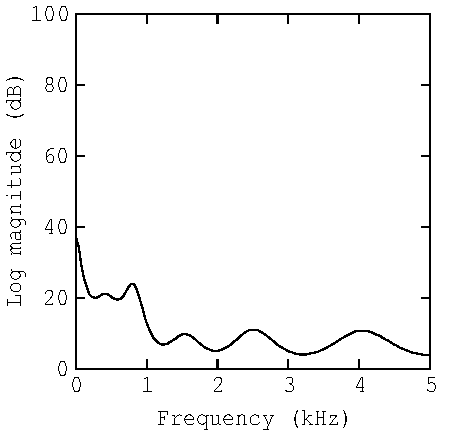
\includegraphics[width=6cm]{fig/mgc2sp.pdf}
\end{center}
\end{qsection}

\begin{qsection}{NOTICE}
The --o option number (the --p option is assigned) is different from
the --q option of mcep and mgcep.
\end{qsection}

\begin{qsection}{SEE ALSO}
\hyperlink{c2sp}{c2sp},
\hyperlink{mgc2mgc}{mgc2mgc},
\hyperlink{gc2gc}{gc2gc},
\hyperlink{freqt}{freqt},
\hyperlink{gnorm}{gnorm},
\hyperlink{lpc2c}{lpc2c}
\end{qsection}
